\section{MPI Load Balancing}
\label{sec:mpi_bal}

To solve the load balance problem, a different strategy is sugested in \cite{paper} to implement the distribution of keys across each processor at the end of each iteration.

The original approach assigns each bucket to one processor. Since bucket have a wide range of sizes, this creates a big inbalance in key distribution. The approach used changes the division process. Each process is first required to receive all information about local bucket counts of all other processors, effectively getting information about how many elements are in every bucket of every process. With this information, a division can be mande across all this information, to equally distribute keys across each processor. \autoref{fig:mpi} illustrates this approach.

\begin{figure}[!htpb]
	\begin{center}
		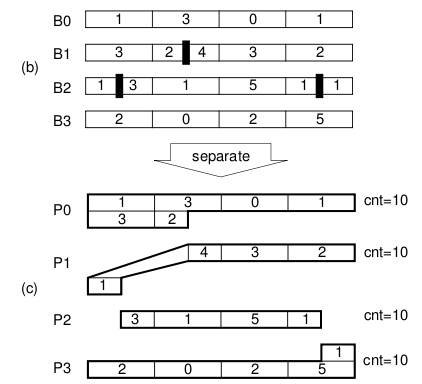
\includegraphics[width=0.45\textwidth]{images/mpi_bal}
	\end{center}
	\caption{An illustration of the load balancing strategy used on the second MPI implementation}
	\label{fig:mpi}
\end{figure}
